%
\section{The model}
\label{sec:model}
The particle content of the model consists of two $SU(2)_L$-doublets of
Weyl fermions $\widetilde{R}_u$, $R_d$  with opposite hypercharges and one singlet
Weyl fermion $N$ of zero hypercharge. 
All of them are odd under one imposed $Z_2$ symmetry, under which the SM
particles are even. 
The new particle content is summarized in Table~\ref{tab:partcont}.
%
\begin{table}
  \centering
  \begin{tabular}{|l|l|l|l|}
    \hline  
    Symbol     & $\left( SU(2)_L, U(1)_Y \right)$ & $Z_2$ & \text{Spin}\\ \hline
    $N$  & $(1,0)$ & $-$ & 1/2\\
     $\widetilde{R}_u$, & $(2, +1/2)$ & $-$ & 1/2\\ 
     $R_d$ & $(2, -1/2)$ & $-$ & 1/2\\ \hline
  \end{tabular}
  \caption{$\alpha$-set of Weyl fermions of the model.}
  \label{tab:partcont}
\end{table}
%
The most general $Z_2$-invariant Lagrangian is given by
\begin{align}
\label{eq:lt13A}
 \mathcal{L}= &\mathcal{L}_{\text{SM}}+\mathcal{L}_{\text{Kin}}+ M_D \epsilon_{ab}R^a_d \widetilde{R}^b_u-\tfrac{1}{2}M_N NN-\lambda_d\, \epsilon_{ab}H^a R_d^b N-\lambda_u \epsilon_{ab}\widetilde{H}^a \widetilde{R}_u^b N+\text{h.c}
\end{align}
where $L_{i}$ are the lepton doublets,  we have defined the new $SU(2)_L$--doublets in terms of left-handed Weyl fermions as
\begin{align}
  R_{d}=&
  \begin{pmatrix}
    \psi_{L}^{0}\\
    \psi_{L}^{-}
  \end{pmatrix}
&  
\widetilde{R}_{u}=&
  \begin{pmatrix}
   - \left( \psi_{R}^{-} \right)^{\dagger}\\
     \left(\psi_{R}^{0}\right)^{\dagger}
  \end{pmatrix},
\end{align}
and $H$ is the SM Higgs doublet with $\widetilde{H}=i\sigma_2H^*$ and $v=246$ GeV.

Using the unitary gauge where  $H=\begin{pmatrix}0 & (h+v)/\sqrt{2}\end{pmatrix}^{\operatorname{T}}$ in the Eq.~\eqref{eq:lt13A} we have
\begin{align}
\label{eq:lt13a-expanded}
\mathcal{L}= &\mathcal{L}_{\text{SM}}+\mathcal{L}_{\text{Kin}}+ M_D(R_d^1\widetilde{R}_u^2-R_d^2\widetilde{R}_u^1)-\tfrac{1}{2}M_N NN
-\lambda_d(H^1R_d^2-H^2R_d^1)N-\lambda_u(\widetilde{H}^1R_u^2-\widetilde{H}^2R_u^1)N+\text{h.c}\nonumber \\
=&\mathcal{L}_{\text{SM}}+\mathcal{L}_{\text{Kin}}+ M_D(\psi_L^0{\psi_{R}^0 }^{\dagger}+\psi_L^-{\psi_{R}^- }^{\dagger})-\tfrac{1}{2}M_N NN
+\dfrac{\lambda_d (h+v)}{\sqrt{2}}\psi_L^0N - \dfrac{\lambda_u (h+v)}{\sqrt{2}}{\psi_R^0}^{\dagger}N +\text{h.c}\nonumber\\
=&\mathcal{L}_{\text{SM}}+\mathcal{L}_{\text{Kin}}+ \left[M_D\psi_L^0{\psi_{R}^0 }^{\dagger}-\tfrac{1}{2}M_N NN + \dfrac{\lambda_d v}{\sqrt{2}}\psi_L^0N - \dfrac{\lambda_u v}{\sqrt{2}}{\psi_R^0}^{\dagger}N\right]
+ M_D\psi_L^-{\psi_{R}^- }^{\dagger}
\nonumber\\ & 
+ \dfrac{h}{\sqrt{2}}\left(\lambda_d\psi_L^0N - \lambda_u{\psi_R^0}^{\dagger}N\right)+\text{h.c}.
%
\end{align}

The $Z_2$-odd fermion spectrum is composed by a
charged Dirac fermion $\chi^-=(\psi^-_L,\, \psi^-_R)^T$ with a tree
level mass $m_{\chi^\pm}=M_D$, and three Majorana fermions $\chi_i^0$ $(i=1,2,3)$ arisen from
the mixture between the neutral parts of the $SU(2)_L$ doublets and
the singlet fermion. 



%%%%%%%%%%%%%%%%%%%%%%%%%%%%%%%%%%%%%%%%%%%%%%%%%%%%%%%%%%%%%%%%%%%%%%%%%%%%%%%%%%%%%%%%%%%%%%%%%%%%%%
\subsection{Neutral mass spectra}
%
By defining the fermion basis through the vector:
\begin{align}
\label{eq:vecgauge}
\boldsymbol{\Xi}^{0}=
\begin{pmatrix}
N & R_d^1 & \widetilde{R}_u^2   
\end{pmatrix}^{\operatorname{T}}=
\begin{pmatrix}
N & \psi_L^0 & \psi_R^{0\dagger}
\end{pmatrix}^{\operatorname{T}},
\end{align} 
the neutral part of the Lagrangian can be writing like
\begin{align}
\label{eq:neutral_lagrangian}
\mathcal{L}_{\Xi}
=& \left[ M_D\psi_L^0{\psi_{R}^0 }^{\dagger}-\tfrac{1}{2}M_N NN
+\dfrac{\lambda_d v}{\sqrt{2}}\psi_L^0N 
- \dfrac{\lambda_u v}{\sqrt{2}} {\psi_R^0}^{\dagger}N\right] +\text{h.c}\nonumber\\
=&-\dfrac{1}{2}\bigg[M_N NN - M_D(\psi_L^0{\psi_{R}^0 }^{\dagger}+{\psi_{R}^0 }^{\dagger}\psi_L^0)
-\dfrac{\lambda_d v}{\sqrt{2}}(\psi_L^0N+N\psi_L^0) 
+\dfrac{\lambda_u v}{\sqrt{2}} ({\psi_R^0}^{\dagger}N+N{\psi_R^0}^{\dagger})\bigg] +\text{h.c}
\nonumber\\
  =&-\frac{1}{2}
\boldsymbol{\Xi}^{0\operatorname{T}}
\mathbf{M}^{\chi}\boldsymbol{\Xi}^0
+\text{h.c}\,,
\end{align}
where
\begin{align}
\label{eq:Mchi}
  \mathbf{M}^{\chi}=\begin{pmatrix}
  M_N                 &-\dfrac{\lambda_d v}{\sqrt{2}}&\dfrac{\lambda_u v}{\sqrt{2}}\\
-\dfrac{\lambda_d v}{\sqrt{2}} &  0                  & -M_D\\
\dfrac{\lambda_u v}{\sqrt{2}}&  -M_D                &  0  \\
\end{pmatrix}\,.
\end{align} 
If we define
%%%%%%%%%%%%%%%%%%%%%%%%%%%%%%%%%%%%%%%%%%%%%%%%%%%%%%%%
\begin{align}
  \label{eq:etabeta}
m_{\lambda}=&  \frac{\lambda v }{\sqrt{2}}\,,&
  \lambda=&\sqrt{\lambda_u^2+\lambda_d^2}\,,&
  \tan\beta=&\frac{\lambda_u}{\lambda_d}\, ,
\end{align}
the neutral fermion mass matrix will be given by
\begin{align}
\label{eq:Mchi}
  \mathbf{M}^{\chi}=\begin{pmatrix}
 M_N                 &-m_{\lambda}\cos\beta&m_{\lambda}\sin\beta\\
-m_{\lambda}\cos\beta &  0                  & -M_D\\
m_{\lambda}\sin\beta&  -M_D                &  0  \\
\end{pmatrix}\,,
\end{align}
which follow the same
convention of the bino-higgsino sector in the neutralino mass matrix of the
minimal supersymmetric standard model (MSSM)~\cite{Martin:2012us}. This convention facilitates the comparison between the present study and previous analysis
regarding the bino-higgsino DM limit of the MSSM. 
Such a limiting scenario occurs in the MSSM when the winos are decoupled from the spectrum and is accommodated within the SDFDM model when
$m_\lambda=m_Z\sin\theta_W$ ($\lambda=g'/\sqrt{2}$).




%%%%%%%%%%%%%%%%%%%%%%%%%%%%%%%%%%%%%%%%%%%%%%%%%%%%%%%%%%%%%%%%%%%%%%%%%%%%%%%%%%%%%%%%%%%%%%%%%
\subsection{Neutral mass eigenstates}
The Majorana fermion mass eigenstates $\mathbf{X}=(\chi_1^0,\chi_2^0,\chi_3^0)^T$ are obtained through the rotation
matrix $\mathbf{N}$\footnote{In~\cite{Horiuchi:2016tqw} we use $\mathbf{U}$ instead $\mathbf{N}$. The equivalence is $\mathbf{N}=\mathbf{U}^T$.} as 

%\begin{align}
%\mathbf{X}= \begin{pmatrix}\chi_1^0\\ \chi_2^0 \\ \chi_3^0\end{pmatrix}
%=\mathbf{U}  \begin{pmatrix}N\\ \psi_L^0 \\ (\psi_R^0)^\dagger\end{pmatrix}=\mathbf{U} \boldsymbol{\Xi}^0\,,
%\end{align}

\begin{align}
\label{eq:rotation}
\boldsymbol{\Xi}^0 = \begin{pmatrix}N\\ \psi_L^0 \\ (\psi_R^0)^\dagger\end{pmatrix}= 
\mathbf{N}\begin{pmatrix}\chi_1^0\\ \chi_2^0 \\ \chi_3^0\end{pmatrix}= \mathbf{N}\mathbf{X}
\end{align}
such that:

\begin{align}
\label{eq:chidiag}
 \mathbf{N}^{\operatorname{T}}\mathbf{M}^\chi \mathbf{N}=\mathbf{M}^\chi_\text{diag}\,,
\end{align}
%The usual suppersymmetric convention is E=N'^{\dagger}X -> N'^{*}M^{\chi}N'^{\dagger}=M^{\chi}_{diag}.
with
$\textbf{M}^\chi_{\text{diag}}=\operatorname{Diag}(m^\chi_1,m^\chi_2,m^\chi_3)$ and $m^\chi_n$ being the corresponding masses (no mass ordering is implied). 
In which follows we assume CP invariance and therefore $\mathbf{N}$ can be chosen real. Therefore, using the neutral Lagrangian Eq.~\eqref{eq:neutral_lagrangian} and the rotation Eq.~\eqref{eq:rotation}  we know that masses will be given by:

\begin{align}
\label{eq:masses_diag}
m^\chi_1=&\tfrac{1}{2}M_NN_{11}^2 - M_D N_{21}N_{31}-\dfrac{\lambda_dv}{\sqrt{2}}N_{11}N_{21}+\dfrac{\lambda_uv}{\sqrt{2}}N_{11}N_{31},\\
m^\chi_2=&\tfrac{1}{2}M_NN_{12}^2 - M_D N_{22}N_{32}-\dfrac{\lambda_dv}{\sqrt{2}}N_{12}N_{22}+\dfrac{\lambda_uv}{\sqrt{2}}N_{12}N_{32},\\
m^\chi_3=&\tfrac{1}{2}M_NN_{13}^2 - M_D N_{23}N_{33}-\dfrac{\lambda_dv}{\sqrt{2}}N_{13}N_{23}+\dfrac{\lambda_uv}{\sqrt{2}}N_{13}N_{33}\,.
\end{align}
%
The analytical diagonalization of the neutral fermion mass matrix is
carried out in Appendix~\ref{sec:analyt-form-mass} 
and for some analysis is convenient to have some approximate expressions in
the limit of small doublet-fermion mixing ($m_\lambda\ll M_D,M_N)$.
Expanding the analytical expressions for the eigensystem of
Eq.~\eqref{eq:chidiag} given in Appendix~\ref{sec:analyt-form-mass}
up to order $m_{\lambda}^2$, the fermion masses are given by
\begin{align}
\label{eq:ml2}
m^\chi_1=&M_{N} + \frac{M_{D} \sin{\left (2 \beta \right )} + M_{N}}{M_{N}^{2}- M_{D}^{2} }\, m_{\lambda}^{2}+\mathcal{O}\left( m_{\lambda}^4 \right) \nonumber\\
m^\chi_2=&M_{D} + \frac{ \sin(2 \beta ) + 1}{2 \left( M_{D} -  M_{N} \right)}\,m_{\lambda}^{2}+\mathcal{O}\left( m_{\lambda}^4 \right) \nonumber\\
m^\chi_3=&- M_{D} + \frac{ \sin(2 \beta ) - 1}{2 \left( M_{D} + M_{N} \right) }\,m_{\lambda}^{2}+\mathcal{O}\left( m_{\lambda}^4 \right)\,.
\end{align}
Approximate expressions for the mixing matrix are also given in the Appendix~\ref{sec:analyt-form-mass}.







%%%%%%%%%%%%%%%%%%%%%%%%%%%%%%%%%%%%%%%%%%%%%%%%%%%%%%%%%%%%%%%%%%%%%%%%%%%%%%%%%%%%%%%%%%%%%%%%%%%%%%%%%%%
\subsection{The interaction's Lagrangian}
%
Using the Lagrangian Eq.~\eqref{eq:lt13a-expanded}, the interaction terms in this model are
%
\begin{align}
\label{eq:lint1}
\mathcal{L} \, \supset \, \mathcal{L}_{\text{Int}}=&\mathcal{L}_{\text{Kin}}
- \dfrac{h}{\sqrt{2}}\left(-\lambda_d\psi_L^0N + \lambda_u{\psi_R^0}^{\dagger}N\right)+\text{h.c}\nonumber\\
= & \dfrac{1}{2}\bar{N}i\slashed{\partial}N + \bar{R_d}i\slashed{D}R_d + \bar{\widetilde{R}_u}i\slashed{D}\widetilde{R}_u
- \dfrac{h}{\sqrt{2}}\left(-\lambda_d\psi_L^0N + \lambda_u{\psi_R^0}^{\dagger}N+\text{h.c}\right)\,,
\end{align}
%
where $\slashed{D}$ is the covariant derivative. 
In the  Appendix~\ref{sec:lag-interaction}
we construct the Majorana spinor $X_i^0$ and the Dirac spinor $X^{\pm}$  as
\begin{align}
X_i^0=\begin{pmatrix}
(\chi_{i}^0)_\alpha \\ (\chi_i^{0\dagger})^{\dot{\alpha}}
\end{pmatrix}
=\begin{pmatrix}
N_{ji}\,\boldsymbol{\Xi}^{0}_j \\
N_{ji}^{\dagger}\,\boldsymbol{{\Xi}^{\dagger}}^{0}_j
\end{pmatrix}
\hspace{1.5 cm}
X^{\pm}=\begin{pmatrix}
\chi^{\pm}_{\alpha} \\ {\chi^{\mp}}^{\dagger\dot{\alpha}}
\end{pmatrix}
=\begin{pmatrix}
\psi_L^{\pm} \\
{\psi_R^{\mp}}^{\dagger}
\end{pmatrix}\,,
\end{align}
%
and we show that the interaction's Lagrangian is given by
%
\begin{align}
\label{eq:lint4}
\mathcal{L}_{\text{Int}}= & 
-\dfrac{g}{\sqrt{2}}\left(\bar{X}^-\slashed{W}\left(N_{2i}P_L-N_{3i}P_R\right)X_i^0 + \text{h.c}\right)
+ \dfrac{g}{4\cos\theta}\bar{X}_i^0\slashed{Z}\left(N_{2i}N_{2j}-N_{3i}N_{3j}\right)\gamma^5X_j^0 \nonumber\\
+& g\left(\dfrac{2\cos^2\theta_W-1}{2\cos\theta_W}\right)
\bar{X}^-\slashed{Z}X^-
-e\bar{X}^-\slashed{A}X^- 
-\dfrac{1}{\sqrt{2}}h\bar{X}_i^0\left(-\lambda_dN_{2i}N_{1j} + \lambda_uN_{3i}N_{1j}\right)X_j^0\,.
\end{align}
%
In particular, the interaction of the DM particle $X_i^0$ with the $W$, $Z$ and $h$ SM gauge boson is given by~\cite{Abdallah:2015ter}
%
\begin{align}
\mathcal{L^{\chi}}_{\text{Int}}=-\bar{X}^-\slashed{W}c_{WXX_i}X_i^0
-c_{ZX_iX_j}Z_{\mu}\bar{X}_i^0\gamma^{\mu}\gamma^{5}X_j^0
-c_{hX_iX_j}h\bar{X}_i^0X_j^0 \,,
\end{align}
where 
\begin{align}
c_{WXX_i}=& \dfrac{g}{\sqrt{2}}\left(N_{2i}P_L-N_{3i}P_R\right)  \label{eq:cWXXi}\\
c_{ZX_iX_j}=&\frac{g}{4\cos\theta_W}(N_{3i}N_{3j}-N_{2i}N_{2j}) \label{eq:cZXiXj}\\
%problema en el orden
c_{hX_iX_j}=&\frac{1}{\sqrt{2}}(-\lambda_dN_{2i}N_{1j}+\lambda_uN_{3i}N_{1j})\label{eq:cHXiXj}\,.
\end{align}
 
As is usually done, we denote the lightest stable particle in our model by $\chi^0$, whose couplings with the $Z$ and $h$ gauge bosons can explicitly written as~\cite{Calibbi:2015nha}
\begin{align}
c_{Z\chi^0\chi^0}&=-\frac{m_Z\lambda^2v(m_{\chi^0}^{2}-M_D^2)\cos2\beta}{2(m_{\chi^0}^{2}-M_D^2)^2+\lambda^2v^2\left(2\sin2\beta m_{\chi^0} M_D+m_{\chi^0}^{2}+M_D^2\right)},\label{eq:cZXX}\\
c_{h\chi^0\chi^0}&=-\frac{(M_D\sin 2\beta+m_{\chi^0})\lambda^2v}{M_D^2+\lambda^2v^2/2+2M_N\,m_{\chi^0}-3m_{\chi^0}^{2}}\label{eq:cHXX}.
\end{align}



%%%%%%%%%%%%%%%%%%%%%%%%%%%%%%%%%%%%%%%%%%%%%%%%%%%%%%%%%%%%%%%%%%%%%%%%%%%%%%
\section{Indirect detection}

%\subsection{DM self-annihilation channels}

\begin{figure}
\begin{center}
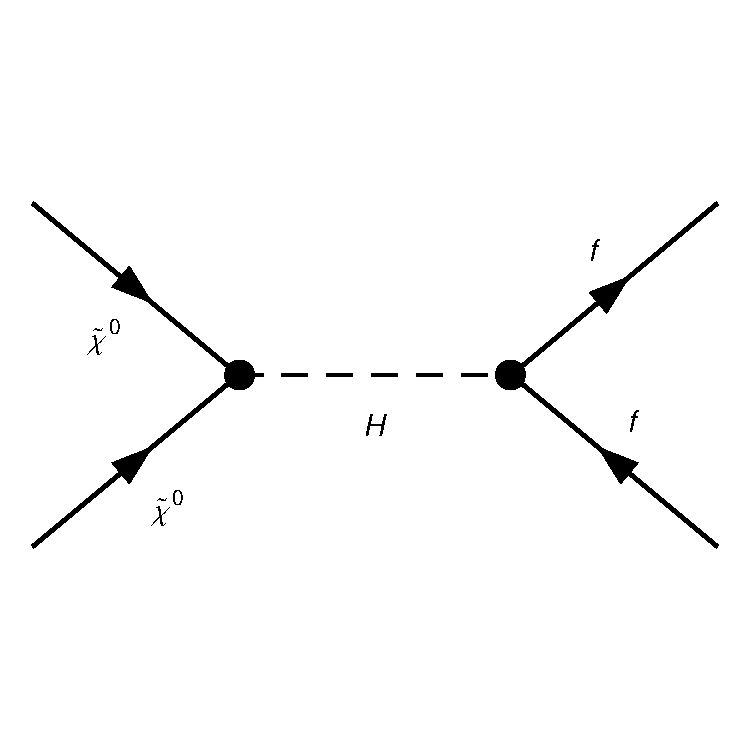
\includegraphics[scale=0.4]{XXHff}
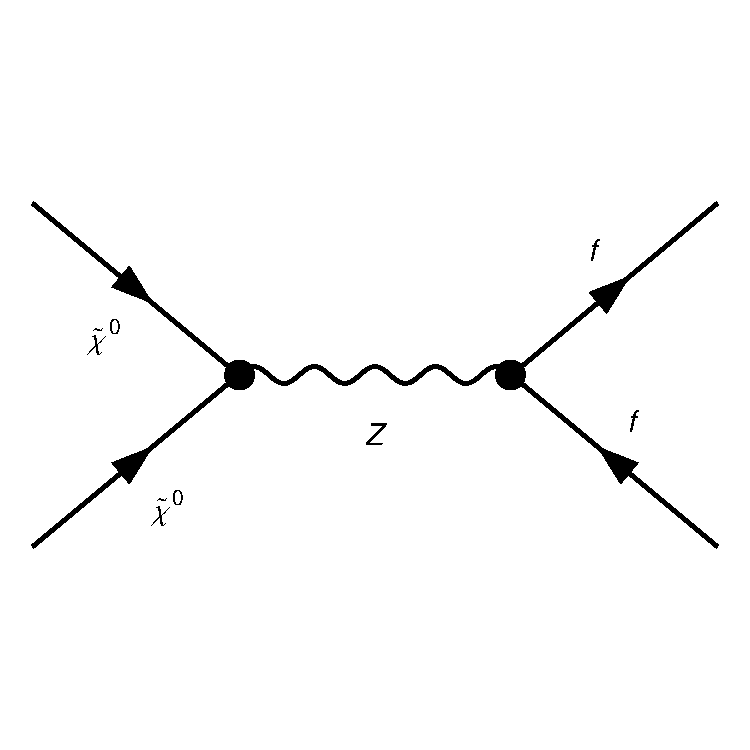
\includegraphics[scale=0.4]{XXZff}
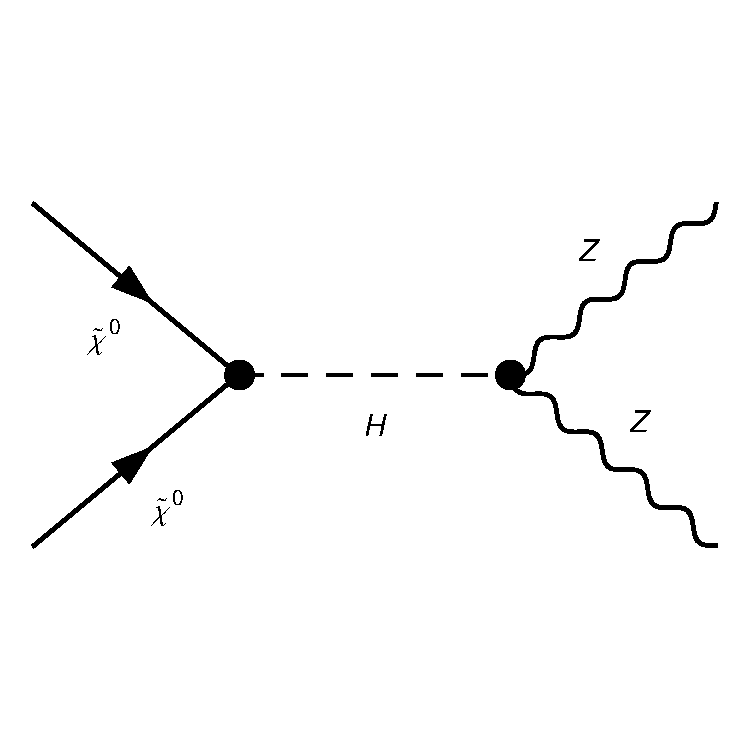
\includegraphics[scale=0.4]{XXHZZ}
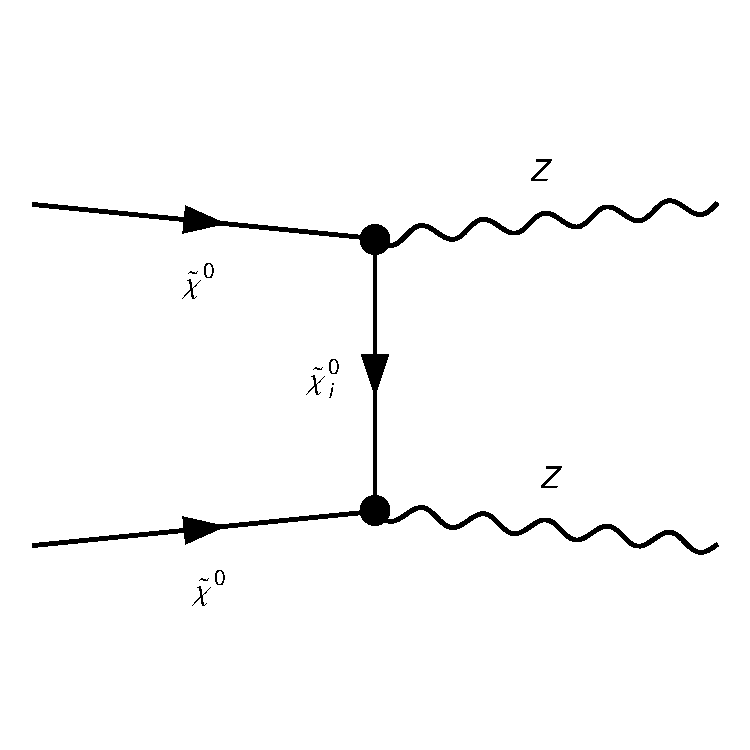
\includegraphics[scale=0.4]{XXXZZ}
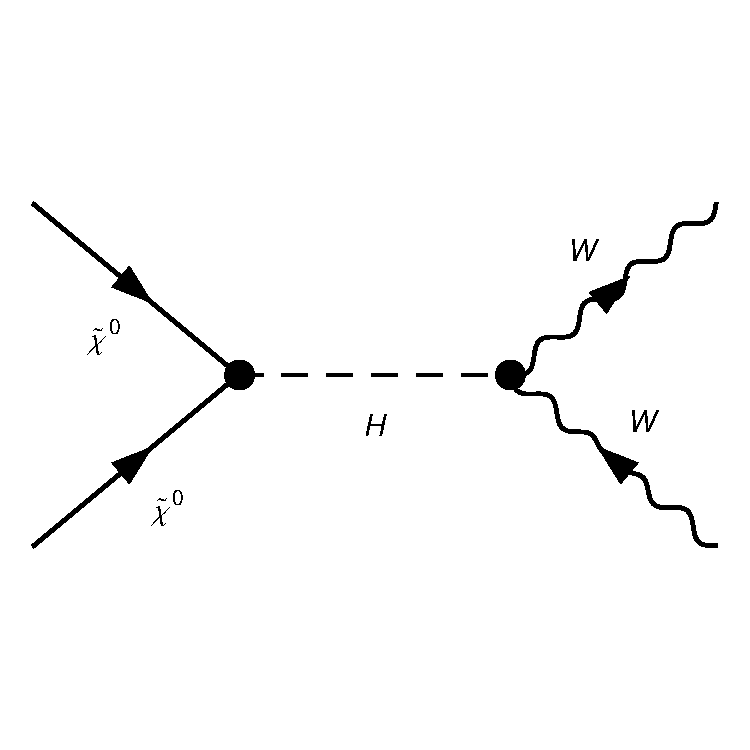
\includegraphics[scale=0.4]{XXHWW}
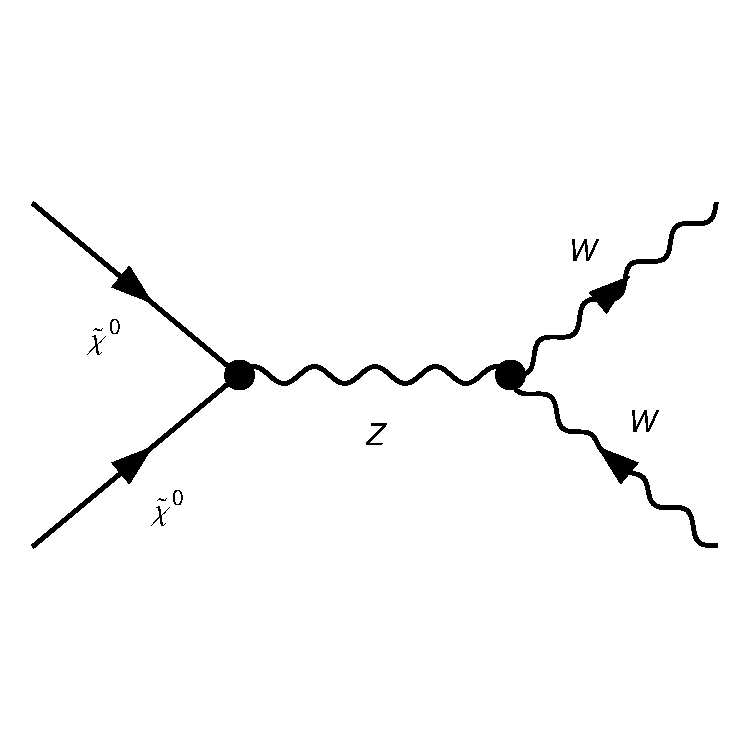
\includegraphics[scale=0.4]{XXZWW}
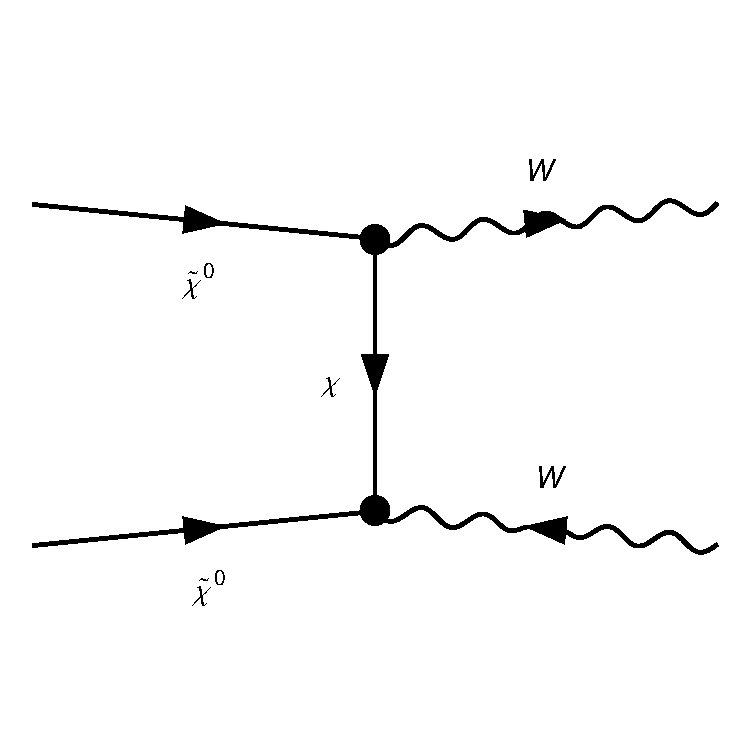
\includegraphics[scale=0.4]{XXXWW}
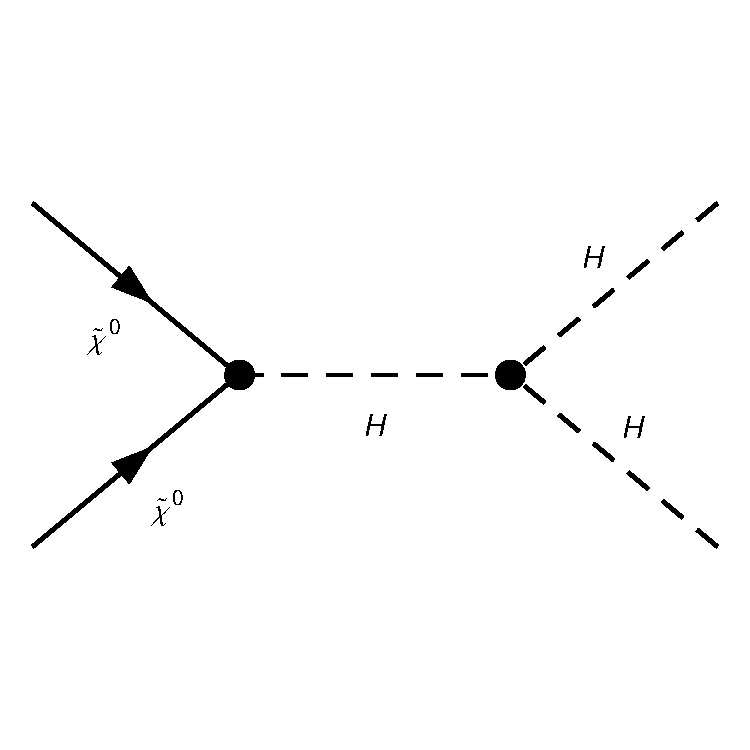
\includegraphics[scale=0.4]{XXHHH}
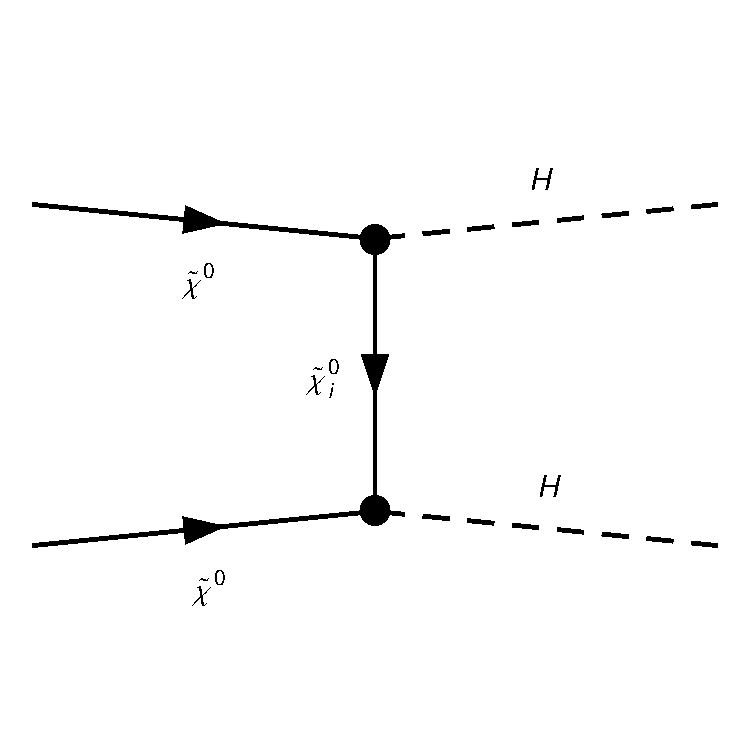
\includegraphics[scale=0.4]{XXXHH}
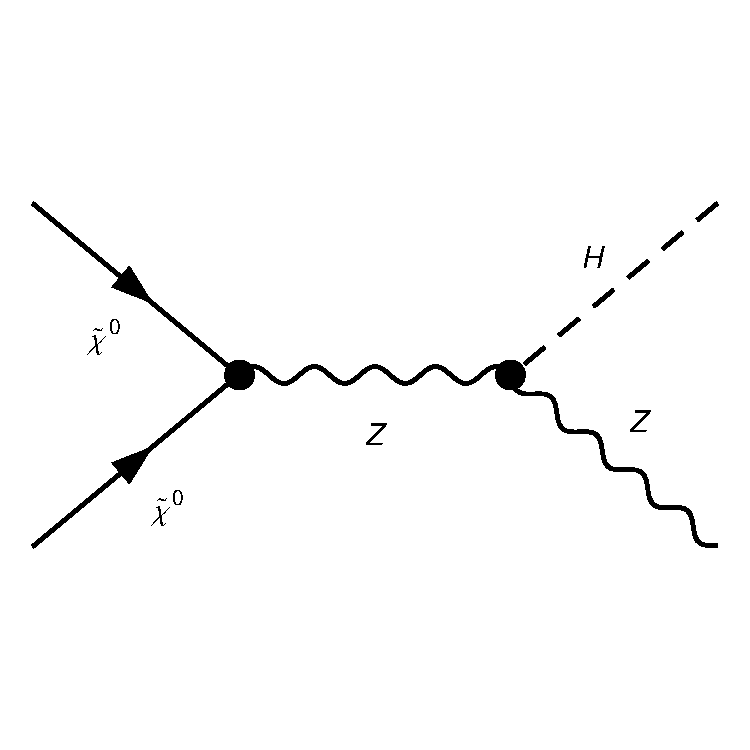
\includegraphics[scale=0.4]{XXZHZ}
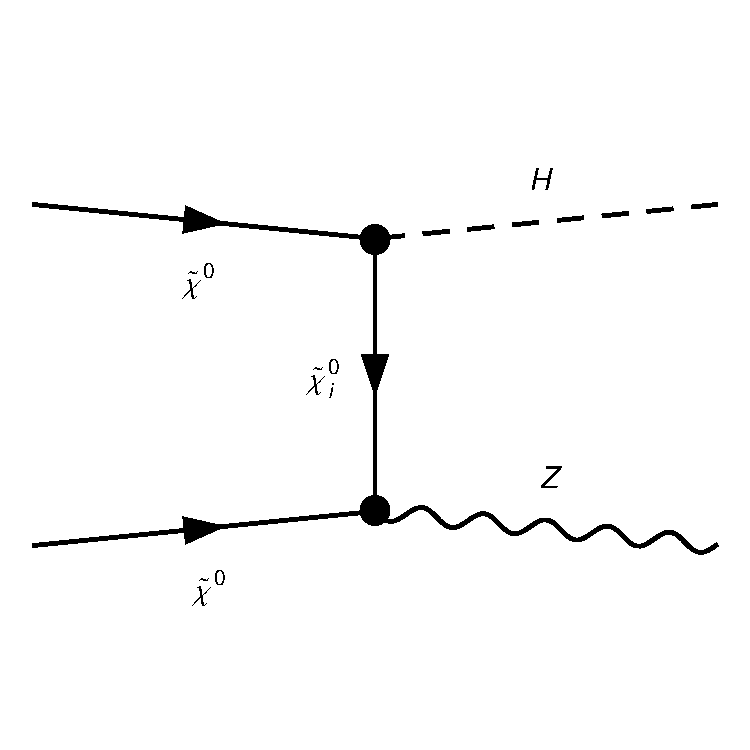
\includegraphics[scale=0.4]{XXXHZ}
\end{center}
\caption{Self-annihilation channels a tree level in the SDFDM model. The u-channels are not shown. They were generated using our implementation in \textsc{FeynArts}~\cite{Hahn:2000kx}.}
\label{fig:self-channels}
\end{figure}

At tree level, the interaction between the DM and the SM sector is mediated by the $W$, $Z$ and $H$ gauge bosons.
In this model, DM particles ($\chi^0$) can self-annihilate into $\bar{f}f$, $ZZ$, $W^+W^-$ and $hh$ final states through  $s$-channel Higgs and $Z$ boson exchange and into $ZZ$, $W^+W^-$ states via $t$-channel $\chi_i^0$ and $\chi^{\pm}$ exchange. Annihilations into a mixture of weak gauge bosons $Zh$ are also possible through the exchange of a $\chi_i\neq\chi^0$  in the $t$-channel or a $Z$ in the $s$-channel. Those annihilations channels are shown in the Fig.~\ref{fig:self-channels}.  We remark in passing that gamma-ray lines $\gamma\gamma$ and $\gamma Z$ can also be produced at one-loop level and it will be extensively discussed in the sec.~\ref{sec:gammarays-SDFDM}. 

Of particular importance for indirect detection studies in this framework is the fact that since DM annihilations into fermion pairs mediated by the Higgs are $p$-wave suppressed (there is no $s$-wave amplitude), the annihilations produced through $Z$ exchange are dominant. We note that the later is also helicity suppressed, this implies that the main annihilation channel is the $t\bar{t}$ ($b\bar{b}$) for a dark matter mass above (below) the top mass, with $\langle\sigma v \rangle\lesssim 10^{-27}$ cm$^3$ s$^{-1}$ for $m_{\chi^0}<m_W$ \cite{Calibbi:2015nha}. 

In the case scenario of DM particles going into gauge bosons, we find that only those processes in the $t$-channel are relevant because they do not suffer velocity suppression. Such a non-velocity suppression is also present in $s$ and $t$ channels for the annihilation into $Zh$. 
In contrast, we get that processes in which DM self-annihilates into a couple of Higgs bosons are velocity suppressed. 

%%%%%%%%%%%%%%%%%%%%%%%% PLOT SV %%%%%%%%%%%%%%%%%%%%%%%%%%%
\begin{figure}[h]
\begin{center}
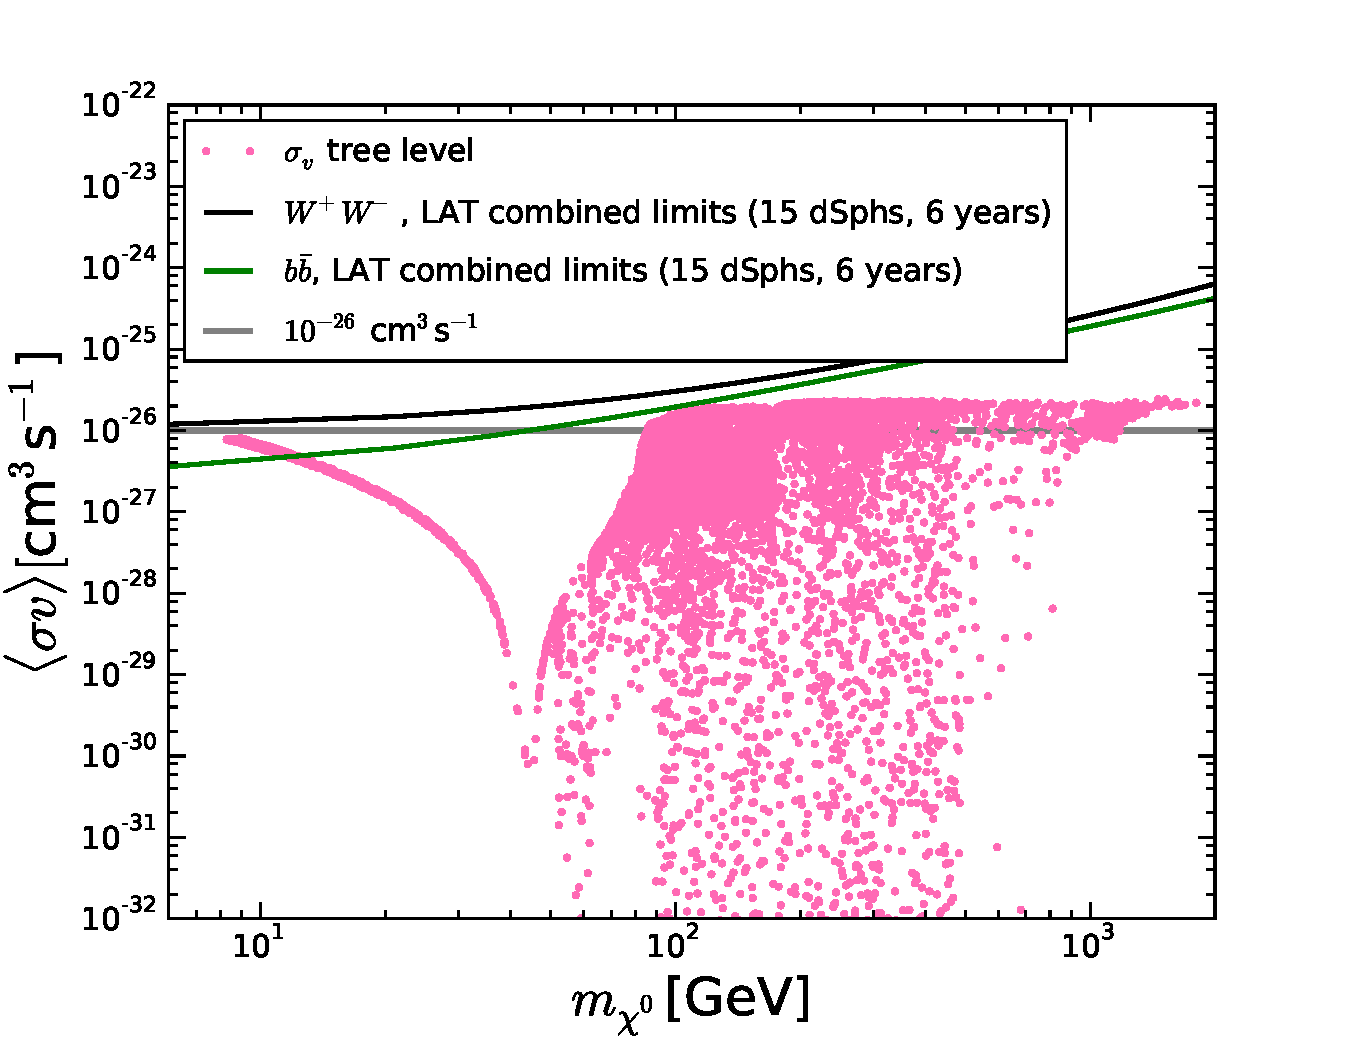
\includegraphics[scale=0.5]{sigmav-T13A}
\end{center}
\caption{Velocity average cross-section $\langle\sigma v\rangle$, generated randomly for a big sample of the parameters of the SDFDM model that take into account the correct relic density (see section~\ref{sec:Parameter-scan}). The green (black) line is the current constraint of indirect detection for DM annihilation into $b\bar{b}$ ($W^+W^-$) in the Dwarf spheroidal galaxies (dSph) at 95$\%$ C.L~\cite{Ackermann:2015zua}. The gray line represent the prediction of the WIMP paradigm where the $\langle\sigma v\rangle$ reach the thermal value $10^{-26}\text{cm}^{3}\text{s}^{-1}$.}
\label{fig:sigmav-random}
\end{figure}
%%%%%%%%%%%%%%%%%%%%%%%%%%%%%%%%%%%%%%%%%%%%%%%%%%%%%%%%%%%%%%%%%

In the Fig.~\ref{fig:sigmav-random} we show the total velocity average cross-section $\langle\sigma v\rangle$ for the self-annihilation of DM into SM particles including two and three final states compute with \textsc{micrOMEGAs 4.1.8}~\cite{Belanger:2014vza} through \textsc{Feynrules 2.3}~\cite{Christensen:2008py}. Each individual model (point) saturates the Planck measurement value for the relic density $\Omega h^2=(0.1199\pm0.0027)$~\cite{Ade:2013zuv} at $3\sigma$ level because we are interested in considering the case where this model accounts for the majority of the DM. It was generate randomly for a big sample of the parameters of the SDFDM model that we will describe latter in the section \ref{sec:Parameter-scan}. Also, we show the current and strogest \textit{Fermi}  Large Area Telescope (LAT) \footnote{\textit{Fermi}  Large Area Telescope: \url{http://fermi.gsfc.nasa.gov/}.} constraints of DM self-annihilation into $b\bar{b}$ quarks and $W^+W^-$ gauge bosons in the Dwarf spheroidal galaxies (dSph)~\cite{Ackermann:2015zua}. We see that indirect detection doesn't put strong constrains for the parameter space of the SDFDM model. All the models are alive with the current indirect detection constrains.    



%%%%%%%%%%%%%%%%%%%%%%%%%%%%%%%%%%%%%%%%%%%%%%%%%%%%%%%%%%%%%%%%%%%%%
\section{Direct detection}
Regarding direct detection, the Higgs $h$ ($Z$ gauge bosson) exchange leads to spin independent (spin dependent) DM nucleon scattering (see Fig.~\ref{fig:SD_SI}). From Eq.~\eqref{eq:cZXX} we get that the spin dependent (SD) cross section vanishes for $\cos2\beta=0$ or $|m_{\chi^0}|=M_D$, implying for both cases that $\tan\beta=\pm1$. In the same vein, from Eq.~\eqref{eq:cHXX} the spin independent (SI) cross section vanishes (i.e. a blind spot as discussed by Ref.~\cite{Cheung:2013dua}) for $\sin2\beta=-m_{\chi^0}/M_D$, which leads to $m_{\chi^0}=M_N, M_D$ using the characteristic equation of the Appendix~\eqref{sec:analyt-form-mass}. Note that $\sigma_{SI}=0$ if $\tan\beta<0$ and that only if $M_N>M_D$ both $\sigma_{SI}$ and $\sigma_{SD}$ can be zero simultaneously. 
%
\begin{figure}[h]
  \centering
  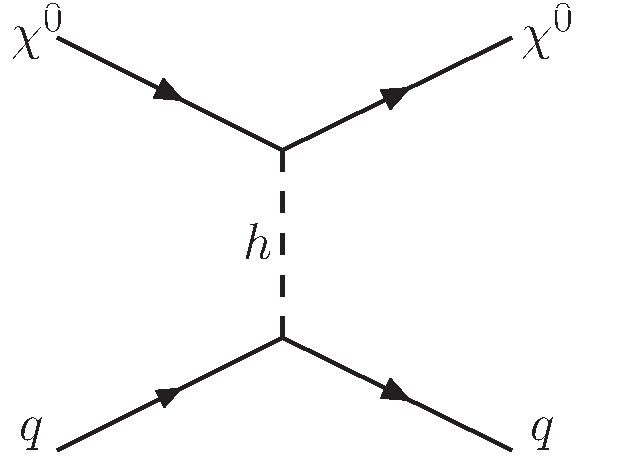
\includegraphics[scale=0.5]{SI} 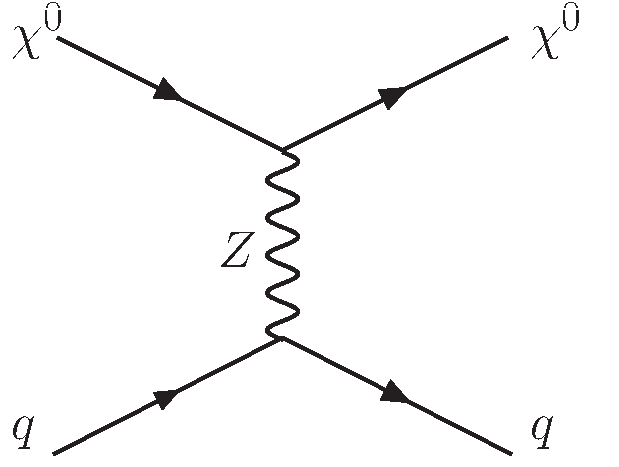
\includegraphics[scale=0.5]{SD}
  \caption{DM inelastic scattering with the quarks that compose the nucleons (protons and neutrons).}
  \label{fig:SD_SI}
\end{figure}





%%%%%%%%%%%%%%%%%%%%%%%%%%%%%%%%%%%%%%%%%%%%%%%%%%%%%%%%%%%%%%%%%%%%%%%%%%%%%%%%%%%%%%%%%%%%%%%%%%%%
\subsection{The spin independent cross section $\sigma_{SI}$}

The last scattering of the DM with the nucleons $N$ (protons and neutrons) is an effective interaction because nucleons are made of quarks. When the mediator is the Higgs gauge boson ($h$), we have an scalar interaction spin independent. In order to compute this scattering is reasonable to think in the next $h$ effective interaction with nucleons  
\begin{align}
\mathcal{L}_{\text{SM}}\supset & \sum_{q}\dfrac{m_q}{v}h\bar{q}q
= |N\rangle\langle N|\sum_{q}\dfrac{m_q}{v}h\bar{q}q |N\rangle\langle N|
= \dfrac{h}{v}\langle N|\sum_{q}m_q\bar{q}q|N\rangle |N\rangle\langle N|
=\dfrac{m_Nf_N}{v}h\bar{N}N\,,
\end{align}
where $\langle N|\sum_{q}m_q\bar{q}q|N\rangle=m_Nf_N$ is a QCD form factor~\cite{Belanger:2014vza},~\cite{Abdallah:2015ter} which is experimentally determined. 

The spin independent cross section a tree level is compute in the Appendix~\ref{sec:SI-amplitude}. It is given by
\begin{align}
\label{eq:SI-tree-level}
\sigma_{SI}=\dfrac{m_r^2}{\pi}\left(\dfrac{c_{hX_1X_1}}{vm_h^2}\right)^2f_N^2m_N^2\,,
\end{align}
%
where $m_r=\dfrac{m_Nm_{\chi^0}}{(m_N+m_{\chi^0})}$
is the DM nucleon reduce mass ($m_N\approx 0.939 \text{GeV}$ for the neutron and $m_N\approx 0.938 \text{GeV}$ for the proton). 

%%%%%%%%%%%%%%%%%%%%%%%%%%%%%%%%%%%% PLOT: SI %%%%%%%%
\begin{figure}[h]
\begin{center}
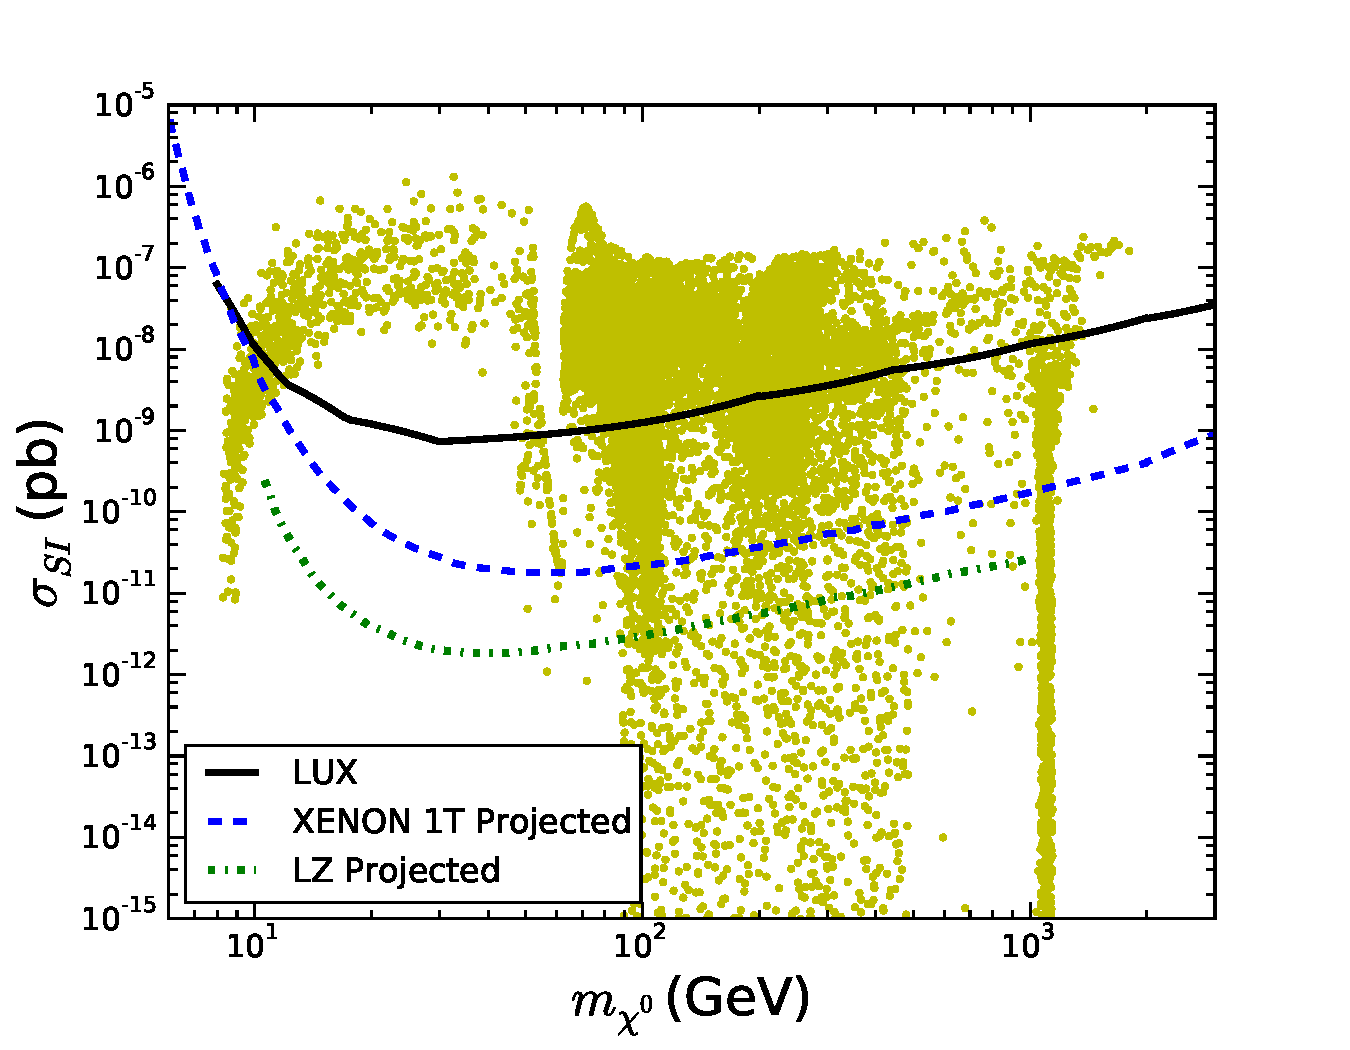
\includegraphics[scale=0.5]{sigmaSI-T13A}  
\caption{Spin-independent $\sigma_{SI}$  direct detection cross sections in the SDFDM model in comparison to current and future direct detection limits. 
The panel displays current limits from the LUX experiment (black solid line)~\cite{2013arXiv1310.8214L} and the expected limits from the forthcoming XENON-1T and LZ~\cite{Cushman:2013zza} experiments (blue dashed and green dot-dashed lines).
}
\label{fig:sigma-SI}
\end{center}
\end{figure}
%%%%%%%%%%%%%%%%%%%%%%%%%%%%%%%%%%%%%%%%%%%%%%%%%%%%%%

In the Fig.~\ref{fig:sigma-SI} we show the spin-independent $\sigma_{SI}$  direct detection cross sections compute with \textsc{micrOMEGAs 4.1.8}~\cite{Belanger:2014vza} through \textsc{Feynrules 2.3}~\cite{Christensen:2008py}. Each individual model (point) saturates the Planck measurement value for the relic density $\Omega h^2=(0.1199\pm0.0027)$~\cite{Ade:2013zuv} at $3\sigma$ level because we are interested in considering the case where this model accounts for the majority of the DM. It was generate randomly for a big sample of the parameters of the SDFDM model that we will describe latter in the section \ref{sec:Parameter-scan}. 
Also, we show the current limits from the LUX experiment (black solid line)~\cite{2013arXiv1310.8214L} and the expected limits from the forthcoming XENON-1T and LZ~\cite{Cushman:2013zza} experiments (blue dashed and green dot-dashed lines.  
We see that direct detection rule out some parameters space of this model. However some of the models are alive with the current direct detection constrains.     



%%%%%%%%%%%%%%%%%%%%%%%%%%%%%%%%%%%%%%%%%%%%%%%%%%%%%%%%%%%%%%%%%%%%%%%%%%%%%%%%%%%%%%%%%%%%%%%%%%%%%%%%%%%
\subsection{The spin dependent cross section $\sigma_{SD}$}

As we say before, when the mediator in the scattering of the DM with nucleons $N$ (protons and neutrons) 
is the $Z$ gauge boson, we have an interaction spin dependent.

%%%%%%%%%%%%%%%%%%%%%%%%%%%%%%%%%%%% PLOT: SD  %%%%%%%%%%%
\begin{figure}[h]
\begin{center}
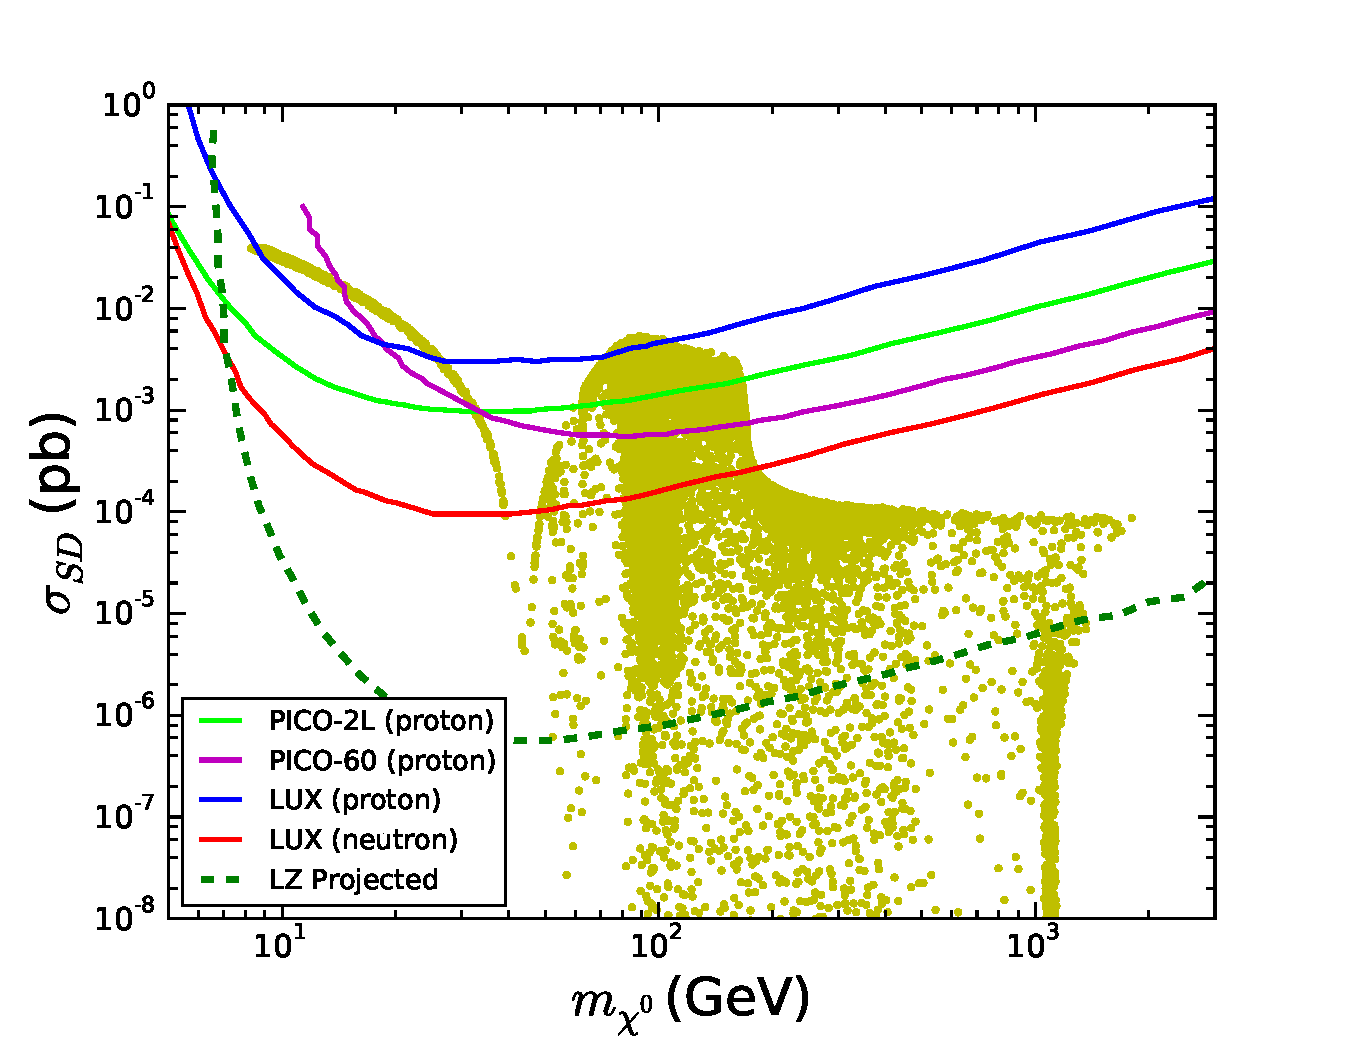
\includegraphics[scale=0.5]{sigmaSD-T13A} 
\caption{Spin-dependent $\sigma_{SD}$ direct detection cross sections in the SDFDM model in comparison to current and future direct detection limits. 
The panel shows the PICO-2L~\cite{Amole:2016pye} (green light solid line) and PICO-60~\cite{Amole:2015pla} (magenta solid line) limits as well as the LZ sensitivity (green dashed line). The most recent constraints from LUX~\cite{Akerib:2016lao} (red and blue solid lines) are also overlaid. 
}
\label{fig:sigma-SD}
\end{center}
\end{figure}
%%%%%%%%%%%%%%%%%%%%%%%%%%%%%%%%%%%%%%%%%%%%%%%%%%%%%%%%%%%%%%%

In the Fig.~\ref{fig:sigma-SD} we show the spin-dependent $\sigma_{SD}$  direct detection cross sections compute with \textsc{micrOMEGAs 4.1.8}~\cite{Belanger:2014vza} through \textsc{Feynrules 2.3}~\cite{Christensen:2008py}. Each individual model (point) saturates the Planck measurement value for the relic density $\Omega h^2=(0.1199\pm0.0027)$~\cite{Ade:2013zuv} at $3\sigma$ level because we are interested in considering the case where this model accounts for the majority of the DM. As we did for the $\sigma_{SI}$, it was compute randomly for a big sample of the parameters of the SDFDM model that we will describe latter in the section \ref{sec:Parameter-scan}. 
Also, we shows the PICO-2L~\cite{Amole:2016pye} (green light solid line) and PICO-60~\cite{Amole:2015pla} (magenta solid line) limits as well as the LZ sensitivity (green dashed line). The most recent constraints from LUX~\cite{Akerib:2016lao} (red and blue solid lines) are also overlaid. 
We see that direct detection rule out some parameters space of this model. However some of the models are alive with the current direct detection constrains, but in the future the LZ experiment will rule out or confirm this model.



%%%%%%%%%%%%%%%%%%%%%%%%%%%%%%%%%%%%%%%%%%%%%%%%%%%%%%%%%%%%%%%%%%%%%%%%%%%%%%%%%%%%%%%%%%%%%%%%%%%%%%%%%%%%
\section{Invisible decays}
In this model we have a new contribution to the Higgs and Z boson invisible decay fraction. Those are given by:

\begin{align}
\Gamma(h \rightarrow \chi\chi) = \dfrac{m_h}{4\pi}\bigg(1-\dfrac{4m_{\chi_1}^2}{m_h^2}\bigg)^{3/2}|c_{h\chi_1\chi_1}|^2
\end{align}
and
\begin{align}
\Gamma(Z \rightarrow \chi\chi) = \dfrac{m_Z}{6\pi}\bigg(1-\dfrac{4m_{\chi_1}^2}{m_Z^2}\bigg)^{3/2}|c_{Z\chi_1\chi_1}|^2 .
\end{align}

Therefore, in order to do a good an viable study in this model, we must to restrict the parameter space to all the points that have a BR($h\rightarrow\chi\chi) < 0.19$ to $2\sigma$ in accord with the LCH an ILC prospects~\cite{Bechtle:2014ewa} and $\Gamma(Z\rightarrow\chi\chi) \lesssim 3$ MeV in accord with LEP~\cite{ALEPH:2005ab}.





%%%%%%%%%%%%%%%%%%%%%%%%%%%%%%%%%%%%%%%%%%%%%%%%%%%%%%%%%%%%%%%%%%%%%%%%%%%%%%%%%%%%%%%%%%%%%%%%%%%%%%%%%%%
\section{STU parameters}
%
In this model, we have new contribution to the EW precision observables (EWPO). The oblique parameters $\Delta S$ and $\Delta T$ have new contributions. The strongest constraints come from $T$ parameters where $\Delta T$ scales as $\sim (\lambda_d^2-\lambda_u^2)^2$ ~\cite{Enberg:2007rp},~\cite{Calibbi:2015nha}. We see that this constraints is important for large $\lambda$ and large $\tan\beta$. We have took care of that.